\documentclass[noauthor,nooutcomes,12pt,hints]{ximera}
\graphicspath{  
{./}
{./whoAreYou/}
{./drawingWithTheTurtle/}
{./bisectionMethod/}
{./circles/}
{./anglesAndRightTriangles/}
{./lawOfSines/}
{./lawOfCosines/}
{./plotter/}
{./staircases/}
{./pitch/}
{./qualityControl/}
{./symmetry/}
{./nGonBlock/}
}


%% page layout
\usepackage[cm,headings]{fullpage}
\raggedright
\setlength\headheight{13.6pt}


%% fonts
\usepackage{euler}

\usepackage{FiraMono}
\renewcommand\familydefault{\ttdefault} 
\usepackage[defaultmathsizes]{mathastext}
\usepackage[htt]{hyphenat}

\usepackage[T1]{fontenc}
\usepackage[scaled=1]{FiraSans}

%\usepackage{wedn}
\usepackage{pbsi} %% Answer font


\usepackage{cancel} %% strike through in pitch/pitch.tex


%% \usepackage{ulem} %% 
%% \renewcommand{\ULthickness}{2pt}% changes underline thickness

\tikzset{>=stealth}

\usepackage{adjustbox}

\setcounter{titlenumber}{-1}

%% journal style
\makeatletter
\newcommand\journalstyle{%
  \def\activitystyle{activity-chapter}
  \def\maketitle{%
    \addtocounter{titlenumber}{1}%
                {\flushleft\small\sffamily\bfseries\@pretitle\par\vspace{-1.5em}}%
                {\flushleft\LARGE\sffamily\bfseries\thetitlenumber\hspace{1em}\@title \par }%
                {\vskip .6em\noindent\textit\theabstract\setcounter{question}{0}\setcounter{sectiontitlenumber}{0}}%
                    \par\vspace{2em}
                    \phantomsection\addcontentsline{toc}{section}{\thetitlenumber\hspace{1em}\textbf{\@title}}%
                     }}
\makeatother



%% thm like environments
\let\question\relax
\let\endquestion\relax

\newtheoremstyle{QuestionStyle}{\topsep}{\topsep}%%% space between body and thm
		{}                      %%% Thm body font
		{}                              %%% Indent amount (empty = no indent)
		{\bfseries}            %%% Thm head font
		{)}                              %%% Punctuation after thm head
		{ }                           %%% Space after thm head
		{\thmnumber{#2}\thmnote{ \bfseries(#3)}}%%% Thm head spec
\theoremstyle{QuestionStyle}
\newtheorem{question}{}



\let\freeResponse\relax
\let\endfreeResponse\relax

%% \newtheoremstyle{ResponseStyle}{\topsep}{\topsep}%%% space between body and thm
%% 		{\wedn\bfseries}                      %%% Thm body font
%% 		{}                              %%% Indent amount (empty = no indent)
%% 		{\wedn\bfseries}            %%% Thm head font
%% 		{}                              %%% Punctuation after thm head
%% 		{3ex}                           %%% Space after thm head
%% 		{\underline{\underline{\thmname{#1}}}}%%% Thm head spec
%% \theoremstyle{ResponseStyle}

\usepackage[tikz]{mdframed}
\mdfdefinestyle{ResponseStyle}{leftmargin=1cm,linecolor=black,roundcorner=5pt,
, font=\bsifamily,}%font=\wedn\bfseries\upshape,}


\ifhandout
\NewEnviron{freeResponse}{}
\else
%\newtheorem{freeResponse}{Response:}
\newenvironment{freeResponse}{\begin{mdframed}[style=ResponseStyle]}{\end{mdframed}}
\fi



%% attempting to automate outcomes.

%% \newwrite\outcomefile
%%   \immediate\openout\outcomefile=\jobname.oc
%% \renewcommand{\outcome}[1]{\edef\theoutcomes{\theoutcomes #1~}%
%% \immediate\write\outcomefile{\unexpanded{\outcome}{#1}}}

%% \newcommand{\outcomelist}{\begin{itemize}\theoutcomes\end{itemize}}

%% \NewEnviron{listOutcomes}{\small\sffamily
%% After answering the following questions, students should be able to:
%% \begin{itemize}
%% \BODY
%% \end{itemize}
%% }
\usepackage[tikz]{mdframed}
\mdfdefinestyle{OutcomeStyle}{leftmargin=2cm,rightmargin=2cm,linecolor=black,roundcorner=5pt,
, font=\small\sffamily,}%font=\wedn\bfseries\upshape,}
\newenvironment{listOutcomes}{\begin{mdframed}[style=OutcomeStyle]After answering the following questions, students should be able to:\begin{itemize}}{\end{itemize}\end{mdframed}}



%% my commands

\newcommand{\snap}{{\bfseries\itshape\textsf{Snap!}}}
\newcommand{\flavor}{\link[\snap]{https://snap.berkeley.edu/}}
\newcommand{\mooculus}{\textsf{\textbf{MOOC}\textnormal{\textsf{ULUS}}}}


\usepackage{tkz-euclide}
\tikzstyle geometryDiagrams=[rounded corners=.5pt,ultra thick,color=black]
\colorlet{penColor}{black} % Color of a curve in a plot



\ifhandout\newcommand{\mynewpage}{\newpage}\else\newcommand{\mynewpage}{}\fi


\title{Dollhouse}
\author{Bart Snapp}

\begin{document}
\begin{abstract}
  Prove to me that you can use your tools by drawing me a dollhouse.
\end{abstract}
\maketitle

\begin{listOutcomes}
\item Apply the constructions from our class.
\item Invent new instructions when needed.
\item Create a plan an carry it through.
\item Disseminate basic mathematical knowledge.
\end{listOutcomes}

Since you've done such great work, you've again been hired (for
points, not hard cash) by the \mooculus\ design company. You see,
now they want someone to design a dollhouse in \snap\ for them.

The dollhouse must have:
\begin{itemize}
\item A reasonable scale ($1'=20$ pixels) and a STAGE of between $360000$
  square pixels and $640000$ square pixels.
\item A plan, or draft, that is drawn and followed along with an
  EXPLANATION of how you used concepts, tools, and so on, from this
  class.
\item At least three rooms. 
\item At least $1$ roof of a given pitch.
\item At least two different sized staircases.
\end{itemize}
For $2$ points extra credit, you could add pets and furniture. But
above all else, \textbf{use the concepts and the BLOCKS from this
  class to draw the dollhouse and EXPLAIN HOW YOU DO THIS.} Show off
your work by showing your PLAN, EXPLAINING how you meet the
requirements of the assignment, and a picture of your final STAGE.



\begin{freeResponse}
  So I chose a scale of $20$ pixels per foot and a Stage of $800\times
  600$ pixels ($480000$ square pixels). My plan is below:
  \begin{center}
    \includegraphics[width=.9\textwidth]{dollhousePlan.pdf}
  \end{center}
  Note that real wall thickness is between $4''$ and $6''$, so I'll
  use $10$ pixels. The ground is at $y=-170$. I used a modified
  bisection method to get the first floor flooring correct. I used an
  ASA block to make the roof. I used the bisection method to find a
  pitch that would work for my plan, and then used a pitch of
  $9/12$. The bisection method was repeatedly used to correct minor
  overlap with the walls/floors.

  Here is my Stage:
  \begin{center}
    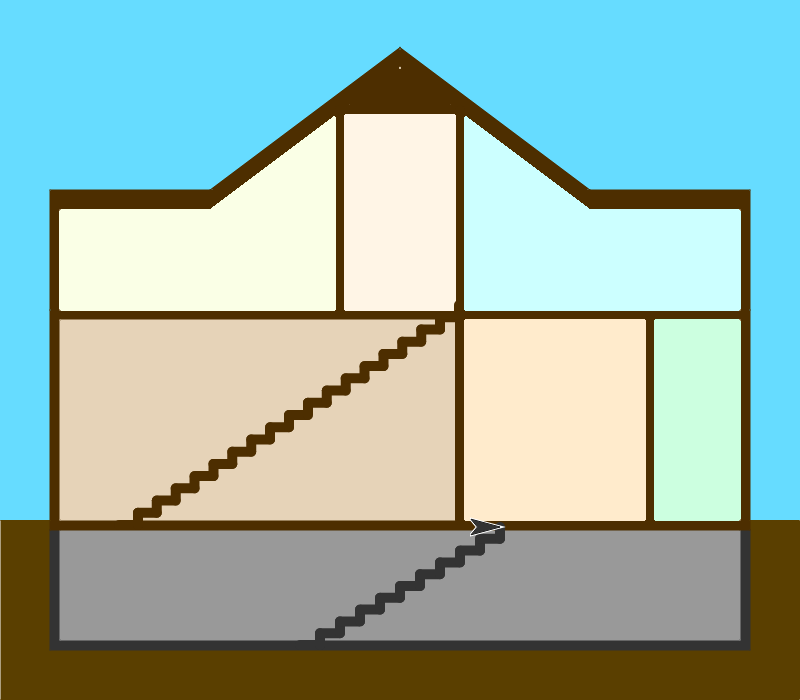
\includegraphics[width=.9\textwidth]{dollhouseStage.png}
  \end{center}
  
  
\end{freeResponse}


\end{document}
